\documentclass[main.tex]{subfiles}
\begin{document}

\section{Introduction}

\subsection{Preliminaries}

We will have convention that for a space time vector $x$ in a chosen frame of reference $\bs{x}$ will mean space part of the vector $x$. $x\cdot y$ will mean Minkowsky inner product:
\begin{equation}
x\cdot y = x^0 y^0 - \bs{x}\cdot \bs{y},
\end{equation}

where $\bs{x}\cdot \bs{y}$ is euclidean inner product in $\R^3$. We will also write $x^2 = x\cdot x$ and $\bs{x}^2 = \bs{x}\cdot\bs{x}.$

When a particle of mass $m$ has a $4$-momentum $p$, 
we will denote it's energy by $E_{\bs{p}} = p^0$. 
Note that

\begin{equation}
E_{\bs{p}} = \sqrt{\bs{p}^2 + m^2}.
\end{equation}

\begin{fact}
If $p, q$ are $4$-momentums of particles of mass $m$, then the expression
\begin{equation}
E_{\bs{q}}\delta^{(3)}(\bs{p} - \bs{q})
\end{equation}
is Lorentz invariant. 
\end{fact}
\begin{proof}
Take Lorentz transformation
\begin{equation}
\begin{cases}
E_{\bs{p}'} = p'^0 = \gamma p^0 - \beta\gamma p^1, \\
p'^1 = \gamma p^1 - \beta\gamma E_{\bs{p}}.
\end{cases}
\end{equation}

Let's calculate 
\begin{multline*}
\\
\delta^{(3)}(\bs{p'} - \bs{q'}) = \delta((p'^1 - q'^1, p'^2 - q'^2, p'^3 - q'^3))\\
= \delta((\gamma p^1 - \beta\gamma E_{\bs{p}} - \gamma q^1 + \beta\gamma E_{\bs{q}},p^2 - q^2, p^3 - q^3)).\\
\\
\end{multline*}
Note that
\begin{equation}
\cfrac{\partial}{\partial p^k} E_{\bs{p}} = \cfrac{\partial}{\partial p^k} \sqrt{\bs{p}^2 + m^2} =
\cfrac{p^k}{E_{\bs{p}}}.
\end{equation}

Then 
\begin{multline*}
\\
\cfrac{\partial}{\partial p^1}(\gamma p^1 - \beta\gamma E_{\bs{p}} - \gamma q^1 + \beta\gamma E_{\bs{q}})\\
\\ = \gamma - \cfrac{\beta\gamma p^1}{E_{\bs{q}}} = \cfrac{E_{\bs{p}}\gamma - \beta\gamma p^1}{E_{\bs{p}}} = \cfrac{E_{\bs{p}'}}{E_{\bs{p}}}.
\\ 
\end{multline*}

Let's write Jacobian

\begin{equation}
\bigg|\cfrac{\partial(\bs{p'} - \bs{q'})}{\partial \bs{p}} \bigg|=
\begin{vmatrix}
\cfrac{E_{\bs{p}'}}{E_{\bs{p}}} & \cfrac{\beta\gamma p^2}{E_{\bs{p}}} & \cfrac{\beta\gamma p^3} 
{E_{\bs{p}}} \\
0 & 1 & 0 \\
0 & 0 & 1
\end{vmatrix} = \cfrac{E_{\bs{p}'}}{E_{\bs{p}}}.
\end{equation}

By Theorem \ref{delta-zeros}, we have
\begin{equation}
 \delta(\bs{p}' - \bs{q}') = \bigg(\bigg|\cfrac{\partial(\bs{p'} - \bs{q'})}{\partial \bs{p}} \bigg|_{\bs{p}=\bs{q}}\bigg)^{-1} \delta(\bs{p} - \bs{q}) =
\cfrac{E_{\bs{q}}}{E_{\bs{q}'}} \delta(\bs{p} - \bs{q}).
\end{equation}




Thus
\begin{equation}
E_{\bs{q}'} \delta^{(3)}(\bs{p'} - \bs{q'}) = E_{\bs{q}}\delta^{(3)}(\bs{p} - \bs{q}).
\end{equation}
\end{proof}

\paragraph{Klein-Gordon equation}

For a relativistic particle $E^2 = \bs{p}^2 + m^2$, there is an idea for relativistic  Schrödinger equation
\begin{equation}
i\hbar \cfrac{\partial}{\partial t}\ket{\phi(t)} =  \sqrt{\bs{P}^2 + m^2} \ket{\phi(t)}.
\end{equation}

which is a motivation for a "squared" version (we will set $\hbar=1$):
\begin{equation}
-\cfrac{\partial^2}{\partial t^2} = \bs{P}^2 + m^2,
\end{equation}
which is
\begin{equation}
-\cfrac{\partial^2}{\partial t^2} = -\nabla^2 + m^2,
\end{equation}
or
\begin{equation}
\cfrac{\partial^2}{\partial t^2} - \nabla^2 + m^2 = 0.
\end{equation} 
Can be noted using raised index of partial derivative and Einstein summation convention:
\begin{equation}
\partial^\mu\partial_\mu + m^2 = 0.
\end{equation}
From this immediately follows Lorentz invariance, but we will give a direct proof in language of tensor transformations Figure \ref{klein-proof}.

\begin{figure}[H]
\label{klein-proof}
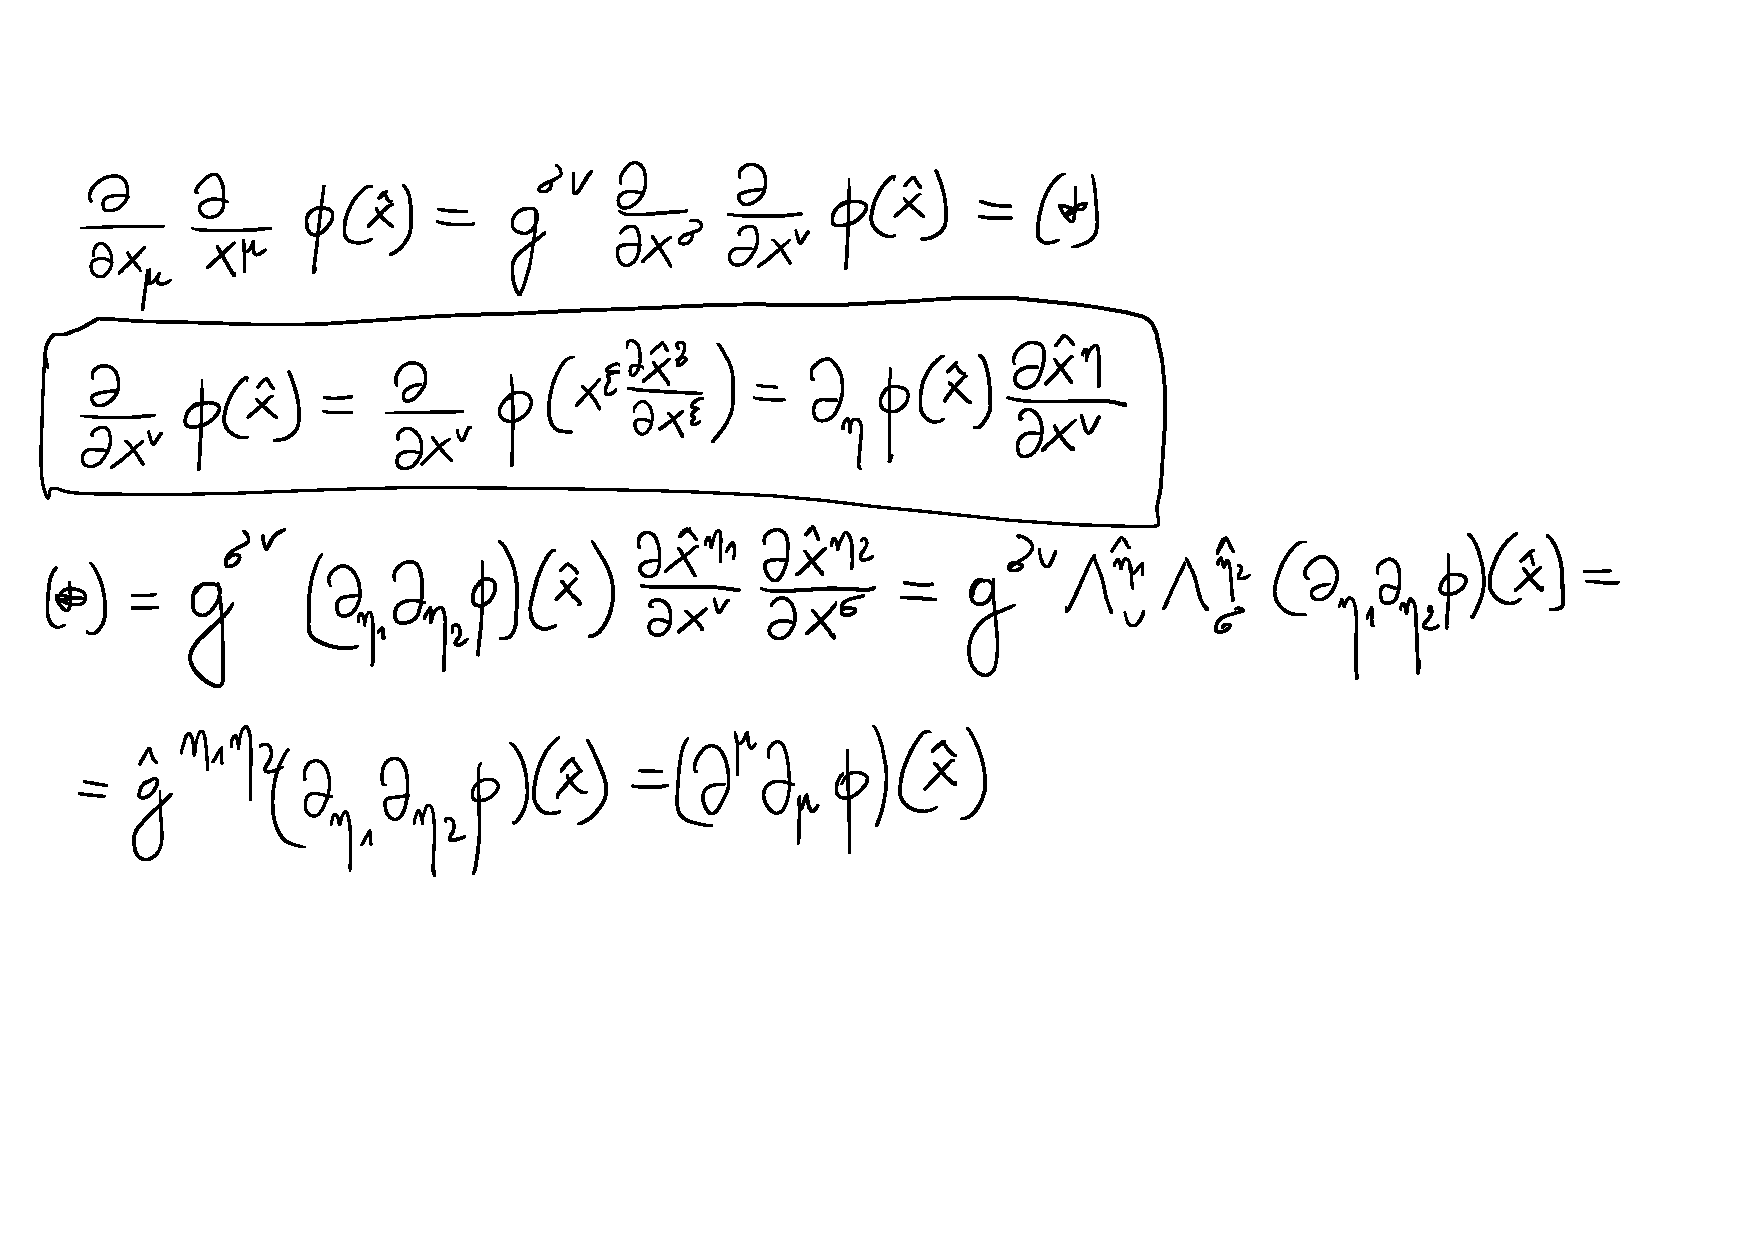
\includegraphics[scale=0.5]{figs/KleinInvariance}
\caption{Proof of Lorentz invariance of Klein-Gordon equation}
\end{figure}


We will often use $\theta$ function as Heaviside step function, defined as follows:

\begin{equation}
\theta(a) = 
\begin{cases}
1 \text{ for } a > 0,\\
0 \text{ for } a < 0.
\end{cases}
\end{equation}

From the physical standpoint $\theta$ is undefined in $0$.

\begin{proposition}
\begin{equation}
\theta(a) = \lim\limits_{\epsilon\to 0^+} \cfrac{i}{2\pi} \int_{-\infty}^\infty  \cfrac{e^{-iax}}{x + i\epsilon} dx
\end{equation}
for $a\not=0$.
\end{proposition}
\begin{proof} This follows imediatelly from Lemma \ref{fourier-residues}.
\end{proof}

It will be also useful to use
\begin{equation}
\label{step-derivative}
\cfrac{d}{da}\theta(a) = \delta(a).
\end{equation}

One of the justifications is the following representation
\begin{equation}
\theta(a) = \int_{-\infty}^a \delta(x) dx.
\end{equation}

If the above seems to be a bit too artificial, let's note that we can also try to argument this from aproximations:

\begin{equation}
\cfrac{d}{da}\bigg(\cfrac{i}{2\pi} \int_{-\infty}^\infty  \cfrac{e^{-iax}}{x + i\epsilon} dx\bigg) = \cfrac{i}{2\pi} \int_{-\infty}^\infty  \cfrac{-i x e^{-iax}}{x + i\epsilon} dx
\xrightarrow[\epsilon \to 0^+]{} \delta(a).
\end{equation}
Ultimetly by this and similiar arguments we can convince ourselves that the equation (\ref{step-derivative}) has enough physical sense. 

We will deal later with Faynman propagators, there is a bit of useful math to work out around it.
Let's take
\begin{equation}
D(z) =  \int \cfrac{d \bs{p}}{(2\pi)^3}
\cfrac{e^{-p \cdot z}}{2E_{\bs{p}}}, 
\end{equation}

where $p = (E_{\bs{p}}, \bs{p})$. Recall $E_{\bs{p}} = \sqrt{\bs{p}^2 + m^2}$.
Let's define 
\begin{equation}
D_F(z) = \theta(z^0)D(z) + \theta(-z^0)D(-z).
\end{equation}

We will show useful (and completly strict mathematically) fact:
\begin{fact}
\begin{equation}
D_F(z) = \lim_{\epsilon\to 0^+}\int \cfrac{d^4 p}{(2\pi)^4} \cfrac{i}{p^2 - m^2 + i\epsilon}\, e^{-ip\cdot z}, 
\end{equation}
where $p$ is just an integration variable over whole spacetime.
\end{fact}
\begin{proof}
Let's calculate
\begin{align}
\label{faynman-propagator-big-integral}
\int \cfrac{d^4 p}{(2\pi)^4} \cfrac{i}{p^2 - m^2 + i\epsilon}\, e^{-ip\cdot z}
= \int \cfrac{e^{i\bs{p}\cdot\bs{z}}d^3 \bs{p}}{(2\pi)^3}
\bigg(-\int_{-\infty}^\infty \cfrac{dp^0}{2\pi i} \cfrac{e^{-ip^0z^0}}{(p^0)^2 - E^2_{\bs{p}} + i\epsilon}\bigg)
\end{align}
Let's concentrate now on the integral in the bracket.
For a fixed $\bs{p}$, lets consider the following representation $E^2_{\bs{p}} - i\epsilon = R_\epsilon e^{-i \omega_\epsilon}$, where $R_\epsilon$ and $\omega_\epsilon$ are real. Note that as we will take $\epsilon \to 0^+$, we will have $R_\epsilon\to E^2_{\bs{p}}$ and $\omega_\epsilon \to 0^+$. Consider square roots of $E^2_{\bs{p}} - i\epsilon$
\begin{align}
& E^{-}_{\bs{p}, \epsilon} = R^{1/2}_\epsilon e^{-i (\omega_\epsilon/2)} \xrightarrow[\epsilon \to 0^+]{} E_{\bs{p}},\\
& E^{+}_{\bs{p}, \epsilon} = R^{1/2}_\epsilon e^{-i (\pi + \omega_\epsilon/2)}
\xrightarrow[\epsilon \to 0^+]{} - E_{\bs{p}}.
\end{align}
It is worth to mention that here the signs for root symbols correspond to the sign of the imaginary part, not to the real part (i.e. they are actually oposit to the sign of the real part). Indeed, since angle $-\omega_\epsilon/2$ is under real axis and $-(\pi + \omega_\epsilon/2)$ is above, we have
\begin{align}
& \Im E^{+}_{\bs{p}, \epsilon} > 0, \\
& \Im E^{-}_{\bs{p},  \epsilon} < 0.
\end{align}
Since the following holds
\begin{equation}
\label{faynman-propagator-small-integral}
\int_{-\infty}^\infty \cfrac{dp^0}{2\pi i} \cfrac{e^{-ip^0z^0}}{(p^0)^2 - E^2_{\bs{p}} + i\epsilon}
= \int_{-\infty}^\infty \cfrac{dp^0}{2\pi i} \cfrac{e^{-ip^0z^0}}{(p^0 - E^{+}_{\bs{p}, \epsilon})(p^0 - E^{-}_{\bs{p}, \epsilon})},
\end{equation}
we can apply Lemma \ref{fourier-residues}.\\
For $z^0 > 0$, the integral (\ref{faynman-propagator-small-integral}) is equal to the minus residuum at pole $E^{-}_{\bs{p},  \epsilon}$, namely:
\begin{equation}
-\cfrac{e^{-i E^{-}_{\bs{p},  \epsilon} z^0}}{E^{-}_{\bs{p},  \epsilon} - E^{+}_{\bs{p},  \epsilon}} \xrightarrow[\epsilon \to 0^+]{} - \cfrac{e^{-i E_{\bs{p}} z^0}}{2E_{\bs{p}}}.
\end{equation}
Thus in limit the integral \ref{faynman-propagator-big-integral} becomes
\begin{equation}
\int \cfrac{e^{i\bs{p}\cdot\bs{z}}d^3 \bs{p}}{(2\pi)^3}
\bigg( \cfrac{e^{-i E_{\bs{p}}z^0 }}{2E_{\bs{p}}} \bigg) = D(z).
\end{equation}


For $z^0 < 0$, the integral (\ref{faynman-propagator-small-integral}) is equal to the residuum at pole $E^{+}_{\bs{p},  \epsilon}$, namely:
\begin{equation}
\cfrac{e^{-i E^{+}_{\bs{p},  \epsilon} z^0}}{E^{+}_{\bs{p},  \epsilon} - E^{-}_{\bs{p},  \epsilon}} \xrightarrow[\epsilon \to 0^+]{} -\cfrac{e^{i E_{\bs{p}} z^0}}{2E_{\bs{p}}}.
\end{equation}
Thus in limit the integral \ref{faynman-propagator-big-integral} becomes
\begin{equation}
\int \cfrac{e^{i\bs{p}\cdot\bs{z}}d^3 \bs{p}}{(2\pi)^3}
\bigg( \cfrac{e^{i E_{\bs{p}}z^0 }}{2E_{\bs{p}}} \bigg) = 
\int \cfrac{e^{-i\bs{p}\cdot\bs{z}}d^3 \bs{p}}{(2\pi)^3}
\bigg( \cfrac{e^{i E_{\bs{p}}z^0 }}{2E_{\bs{p}}} \bigg) = D(-z).
\end{equation}
When we collect cases together, we are getting
\begin{equation}
D_F(z) = \theta(z^0)D(z) + \theta(-z^0)D(-z). 
\end{equation}
\end{proof}


\subsection{Creation and anihilation algebra for bozons and fermions}
In this subsection $p$ indexes are arbitrary and they are not necesarlily related to momentum. 

We are still in a ``usual" Dirac formulation of quantum mechanics. We simply make certain assumptions about family of operators $a_p$ and one distinguished state    $\ket{0} \not= 0$, which is called a vaccume state.

\begin{definition}[Bozonic creation and anihilation assumptions]
We will call the bellow statements \textit{bozonic creation and anihilation assumptions}
\begin{align}
& [a_p, a^\dagger_q] = \delta(p - q),\\
& [a_p, a_q] = 0 \text{ and } [a^\dagger_p, a^\dagger_q] = 0,\\
& a_p\ket{0} = 0.
\end{align}
\end{definition}

\begin{proposition}
Under bozonic creation and anihilation assumptions, we have
\begin{equation}
\label{anihilation-operator-characteristic}
a_p (a_{q_1}^\dagger \dots a_{q_n}^\dagger) = \sum_{k=1}^n\delta(p - q_k) a_{q_1}^\dagger a_{q_{k - 1}}^\dagger \dots a_{q_{k + 1}}^\dagger a_{q_n}^\dagger + (a_{q_1}^\dagger \dots a_{q_n}^\dagger)a_p.
\end{equation}
\end{proposition}
\begin{proof}
Note that (\ref{anihilation-operator-characteristic}) holds for $n = 1$. We will prove it by induction. Let's now assume (\ref{anihilation-operator-characteristic}) holds for $n - 1$.
\begin{align*}
& a_p (a_{q_1}^\dagger \dots a_{q_n}^\dagger)=
a_{q_1}^\dagger a_p (a_{q_2}^\dagger \dots a_{q_n}^\dagger) + \delta(p - q_1) (a_{q_2}^\dagger \dots a_{q_n}^\dagger)= \\
& a_{q_1}^\dagger\sum_{k=2}^n\delta(p - q_k) a_{q_2}^\dagger a_{q_{k - 1}}^\dagger \dots a_{q_{k + 1}}^\dagger a_{q_n}^\dagger + \delta(p - q_1) (a_{q_2}^\dagger \dots a_{q_n}^\dagger) + a_{q_1}^\dagger (a_{q_2}^\dagger \dots a_{q_n}^\dagger)a_p.
\end{align*} 
\end{proof}

\begin{corollary}
\begin{equation}
a_p (a_{q_1}^\dagger \dots a_{q_n}^\dagger) \ket{0} = \sum_{k=1}^n\delta(p - q_k) a_{q_1}^\dagger a_{q_{k - 1}}^\dagger \dots a_{q_{k + 1}}^\dagger a_{q_n}^\dagger \ket{0}.
\end{equation}
\end{corollary}

\begin{corollary}
\begin{equation}
a_p (a_{q}^\dagger)^n \ket{0} = n \delta(p - q) (a_{q}^\dagger)^{n-1} \ket{0}.
\end{equation}
\end{corollary}

\begin{lemma}
If $[a_p, a^\dagger_q] = \delta(p - q)$, then
\begin{align*}
&\int K_1(\dots, p, q, \dots) a_p a^\dagger_q K_2(\dots, p, q, \dots) d \dots dpdq \ldots = \\
&\int K_1(\dots, p, q, \dots) a^\dagger_q a_p K_2(\dots, p, q, \dots) d \dots dpdq \ldots + \\ 
&\int K_1(\dots, p, p, \dots)K_2(\dots, p,p, \dots)d \dots dp \dots.
\end{align*}
\end{lemma}

\begin{proposition} We assume bozonic creation and anihilation assumptions.
Let $F = \int dp\, f(p)a^\dagger_p a_p$ and $G = \int dp\, g(p)a^\dagger_p a_p$, then
\begin{equation}
[F, G] = 0.
\end{equation} 
\end{proposition}
\begin{proof}
\begin{align*}
&FG = \int dp dq \,f(p)g(q) a^\dagger_p a_p a^\dagger_q a_q = \\
& \int dp dq f(p)g(q) a^\dagger_p  a^\dagger_q a_p a_q + \int dp f(p)g(p) a^\dagger_p a_p =  \\
& \int dp dq f(p)g(q) a^\dagger_q a^\dagger_p  a_q  a_p  + \int dp f(p)g(p) a^\dagger_p a_p \\ =
& \int dp dq f(p)g(q) a^\dagger_q a_q a^\dagger_p   a_p - \cancel{\int dq f(q)g(q) a^\dagger_q    a_q}  + \cancel{\int dp f(p)g(p) a^\dagger_p a_p} 
= GF. \\ 
\end{align*}
\end{proof}

\begin{proposition}
We assume bozonic creation and anihilation assumptions. Let $P = \int pdp\, a^\dagger_p a_p$ and
\begin{equation}
\hat{V} = \int dp_1 dp_2 dq\, V_q a^\dagger_{p_1 + q} a^\dagger_{p_2 - q} a_{p_2}a_{p_1}, 
\end{equation}
then $[\hat{V}, P] = 0.$
\end{proposition}
\begin{proof}
Let's do calculations:
\begin{figure}[H]
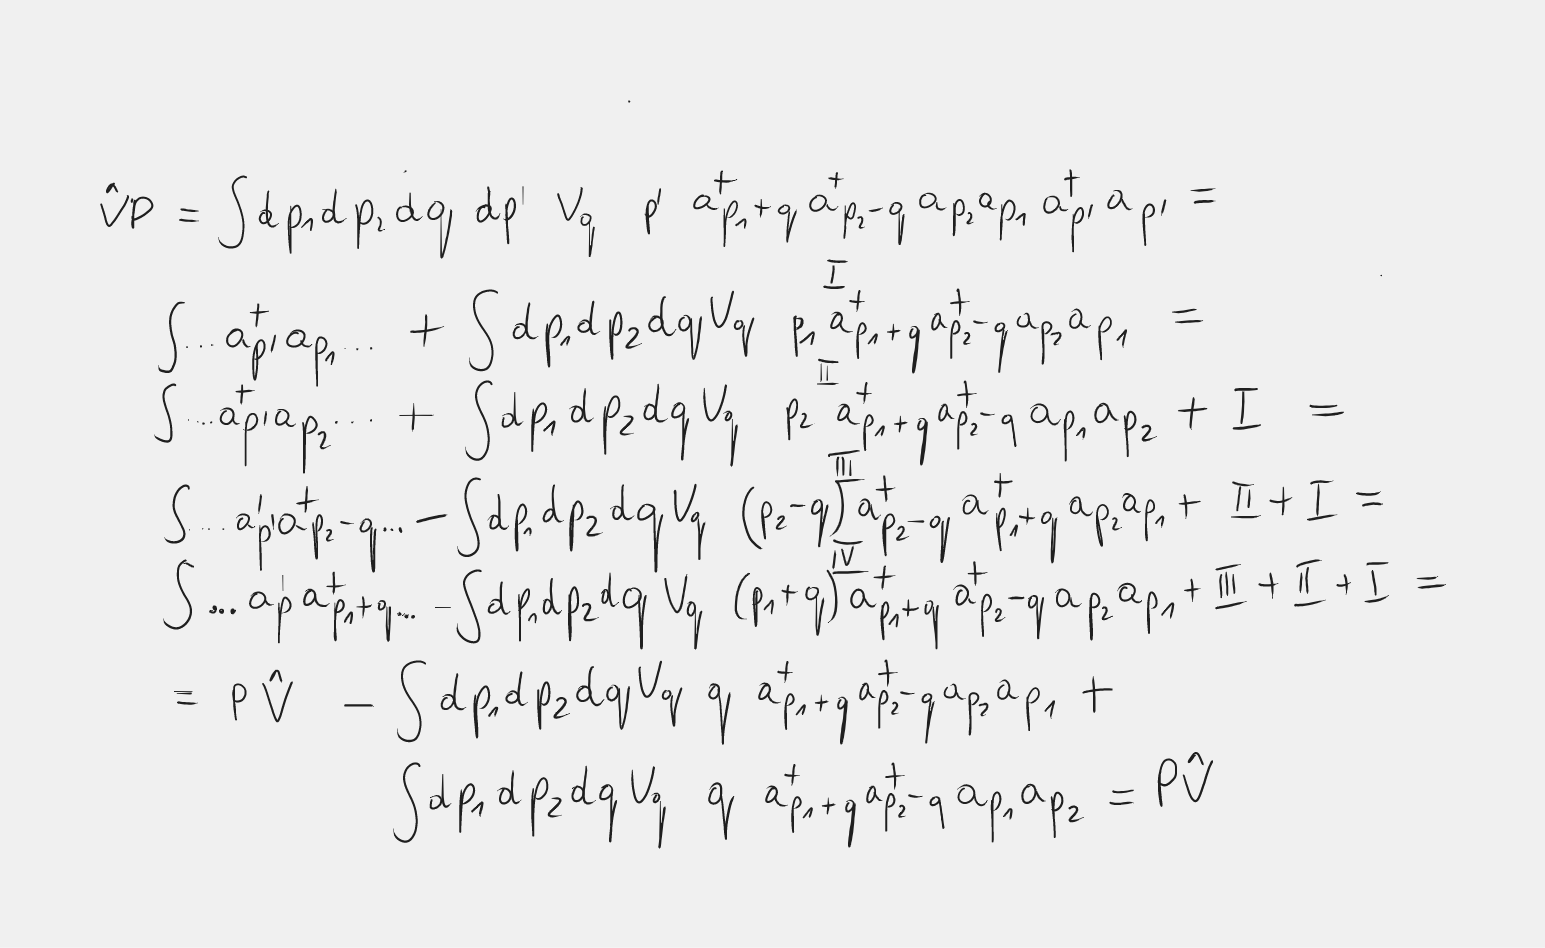
\includegraphics[width=\textwidth]{figs/two_body_potential}
\end{figure}

\end{proof}

Let's now work out a more generic equations which will work with bozons as well as with fermions. For that it will be usefull to introduce a generic commutator expression
\begin{equation}
[A, B]_{\zeta} \stackrel{def}{=} AB -\zeta BA.
\end{equation}

Note that for commutator, we have $[A, B] = [A, B]_1$ and for anticommutator, we have $\{A, B\} = [A, B]_{-1}$.

Note a usefull transposition:
\begin{equation}
AB = [A, B]_{\zeta} + \zeta BA.
\end{equation}

\begin{assumption}
\label{anihilation-creation-assumptions}
Let $\zeta\in\{-1, 1\}$. Assume that the bellow conditions holds for a family of operators $a_p$.
\begin{align}
& [a_p, a^\dagger_q]_\zeta = \delta(p - q),\\
& [a_p, a_q]_\zeta = 0 \text{ and } [a^\dagger_p, a^\dagger_q]_\zeta = 0,\\
& a_p\ket{0} = 0.
\end{align}
\end{assumption}

For $\zeta = 1$ the above are \textit{bozonic anihilation and creation assumptions}, for $\zeta = -1$ the above are \textit{fermionic anihilation and creation assumptions}.

Note that under Assumption \ref{anihilation-creation-assumptions}, we have always

\begin{equation}
a_p a_{q}^\dagger = \delta(p - q) + \zeta a_{q}^\dagger a_p,
\end{equation}

\begin{equation}
a_{q}^\dagger a_p = \zeta \delta(p - q) - \zeta a_p a_{q}^\dagger,
\end{equation}

\begin{equation}
a_p a_q = \zeta a_q a_p,
\end{equation}

\begin{equation}
a^\dagger_p a^\dagger_q = \zeta a^\dagger_q a^\dagger_p.
\end{equation}  

Note that it follows that for fermions we have $a^\dagger_p a^\dagger_p = 0$. For all subsequent calculations it is also worth to remeber that $\zeta^{2k} = 1$ for any integer $k$.

\begin{proposition}
Under Assumption \ref{anihilation-creation-assumptions}, we have
\begin{equation}
\label{anihilation-operator-characteristic}
a_p (a_{q_1}^\dagger \dots a_{q_n}^\dagger) = \sum_{k=1}^n \zeta^{k - 1} \delta(p - q_k) a_{q_1}^\dagger \dots a_{q_{k - 1}}^\dagger a_{q_{k + 1}}^\dagger  \dots  a_{q_n}^\dagger + \zeta^n( a_{q_1}^\dagger \dots a_{q_n}^\dagger)a_p.
\end{equation}
\end{proposition}
\begin{proof}
Note that (\ref{anihilation-operator-characteristic}) holds for $n = 1$. We will prove it by induction. Let's now assume (\ref{anihilation-operator-characteristic}) holds for $n - 1$.
\begin{align*}
& a_p (a_{q_1}^\dagger \dots a_{q_n}^\dagger)=
\zeta a_{q_1}^\dagger a_p (a_{q_2}^\dagger \dots a_{q_n}^\dagger) + \delta(p - q_1) (a_{q_2}^\dagger \dots a_{q_n}^\dagger)= \\
& \zeta a_{q_1}^\dagger\sum_{k=2}^n\zeta^k \delta(p - q_k) a_{q_2}^\dagger \dots a_{q_{k - 1}}^\dagger a_{q_{k + 1}}^\dagger  \dots a_{q_n}^\dagger + \zeta^0 \delta(p - q_1) (a_{q_2}^\dagger \dots a_{q_n}^\dagger) \\
& + \zeta a_{q_1}^\dagger \zeta^{n - 1}(a_{q_2}^\dagger \dots a_{q_n}^\dagger)a_p = \\
& \sum_{k=1}^n \zeta^{k - 1} \delta(p - q_k) a_{q_1}^\dagger a_{q_{k - 1}}^\dagger \dots a_{q_{k + 1}}^\dagger a_{q_n}^\dagger + \zeta^n( a_{q_1}^\dagger \dots a_{q_n}^\dagger)a_p.
\end{align*} 
\end{proof}

\begin{corollary}
Under Assumption \ref{anihilation-creation-assumptions}, we have
\begin{equation}
a_p (a_{q_1}^\dagger \dots a_{q_n}^\dagger) \ket{0} = \sum_{k=1}^n\zeta^{k-1} \delta(p - q_k) a_{q_1}^\dagger \dots a_{q_{k - 1}}^\dagger a_{q_{k + 1}}^\dagger  \dots a_{q_n}^\dagger \ket{0}.
\end{equation}
\end{corollary}

\begin{proposition}
\label{count-operators}
Under Assumption \ref{anihilation-creation-assumptions} for $F = \int dp\, f(p)a^\dagger_p a_p$, we have
\begin{equation}
F a^\dagger_{p_1} \dots a^\dagger_{p_n}\ket{0} = \bigg( \sum_{k = 1}^n f(p_k)\bigg) a^\dagger_{p_1}  \dots a^\dagger_{p_n}\ket{0}.
\end{equation}
\end{proposition}
\begin{proof}
\begin{align*}
& F a^\dagger_{p_1} \dots a^\dagger_{p_n}\ket{0} = \int dp\, f(p)a^\dagger_p a_p a^\dagger_{p_1}  \dots a^\dagger_{p_n}\ket{0} = \\
& \sum_{k=1}^n\zeta^{k-1} f(a_{p_k}) a^\dagger_{p_k}
a^\dagger_{p_1} \tdots \cancel{a^\dagger_{p_k}} \tdots a^\dagger_{p_n}\ket{0} = \\
& \sum_{k=1}^n\zeta^{k-1} \zeta^{k-1} f(a_{p_k}) a^\dagger_{p_1}  \dots a^\dagger_{p_n}\ket{0} = \\
& \bigg( \sum_{k = 1}^n f(p_k)\bigg) a^\dagger_{p_1}  \dots a^\dagger_{p_n}\ket{0}.
\end{align*}
\end{proof}

\begin{proposition} Under Assumption \ref{anihilation-creation-assumptions}, for
$F = \int dp\, f(p)a^\dagger_p a_p$ and $G = \int dp\, g(p)a^\dagger_p a_p$, we have
\begin{equation}
[F, G] = 0.
\end{equation} 
\end{proposition}
\begin{proof}
\begin{align*}
&FG = \int dp dq \,f(p)g(q) a^\dagger_p a_p a^\dagger_q a_q = \\
& \zeta \int dp dq \, f(p)g(q) a^\dagger_p  a^\dagger_q a_p a_q + \int dp\, f(p)g(p) a^\dagger_p a_p =  \\
& \zeta \int dp dq\, f(p)g(q) a^\dagger_q a^\dagger_p  a_q  a_p  + \int dp\, f(p)g(p) a^\dagger_p a_p \\ =
& \zeta \big( \zeta \int dp dq\, f(p)g(q) a^\dagger_q a_q a^\dagger_p   a_p - \zeta \int dq\, f(q)g(q) a^\dagger_q    a_q \big)  + \int dp\, f(p)g(p) a^\dagger_p a_p = \\
& \int dp dq\, f(p)g(q) a^\dagger_q a_q a^\dagger_p   a_p - \cancel{\int dq \, f(q)g(q) a^\dagger_q    a_q}  + \cancel{\int dp\, f(p)g(p) a^\dagger_p a_p} 
= GF. \\ 
\end{align*}
\end{proof}

We will know chnage $p, q$ notation to $\alpha, \beta$ (it is just notation change).

\begin{proposition}
\label{2-particle-potentcial}
Under Assumption \ref{anihilation-creation-assumptions}, for an operator defined as
\begin{equation}
V = \int d\alpha d\beta\, v(\alpha, \beta) a_{\alpha}^\dagger a_{\beta}^\dagger a_{\beta} a_{\alpha},
\end{equation}
we have
\begin{equation}
V a^\dagger_{\alpha_1} \dots a^\dagger_{\alpha_n}\ket{0} = \bigg(\sum_{k\not=k'}v(\alpha_k, \alpha_{k'})\bigg) a^\dagger_{\alpha_1} \dots a^\dagger_{\alpha_n}\ket{0}.
\end{equation}
\end{proposition}
\begin{proof}
\begin{align*}
& V a^\dagger_{\alpha_1} \dots a^\dagger_{\alpha_n}\ket{0} = \int d\alpha d\beta\, v(\alpha, \beta) a_{\alpha}^\dagger a_{\beta}^\dagger a_{\beta} a_{\alpha} a^\dagger_{\alpha_1} \dots a^\dagger_{\alpha_n}\ket{0} = \\
& \sum_{k = 1}^n \zeta^{k - 1} \int d\beta\, v(\alpha_k, \beta)a_{\alpha_k}^\dagger a_{\beta}^\dagger a_{\beta} (a^\dagger_{\alpha_1} \tdots \cancel{a^\dagger_{\alpha_k}} \tdots a^\dagger_{\alpha_n})\ket{0} = \\
& \sum_{k = 1}^n \zeta^{k - 1}\bigg( \sum_{k'=1}^{k - 1} \zeta^{k' - 1}  + \sum_{k'=k+1}^{n} \zeta^{k'}\bigg) v(\alpha_k, \alpha_{k'})a_{\alpha_k}^\dagger a_{\alpha_{k'}}^\dagger (a^\dagger_{\alpha_1} \tdots \cancel{a^\dagger_{\alpha_k}} \cancel{a^\dagger_{\alpha_{k'}}}\tdots a^\dagger_{\alpha_n})\ket{0} = \\
& \sum_{k = 1}^n \zeta^{k-1} \zeta^{k - 1}\bigg( \sum_{k'=1}^{k - 1} \zeta^{k'- 1}\zeta^{k' - 1}  + \sum_{k'=k+1}^{n} \zeta^{k'} \zeta^{k'}\bigg) v(\alpha_k, \alpha_{k'})
a^\dagger_{\alpha_1} \tdots a^\dagger_{\alpha_n}\ket{0} = \\
& \bigg(\sum_{k\not=k'}v(\alpha_k, \alpha_{k'})\bigg) a^\dagger_{\alpha_1} \dots a^\dagger_{\alpha_n}\ket{0}.
\end{align*}
\end{proof}

\subsection{Assembly of identical particles}

Assume we have a space of quantum states $\mathcal{X}$ which desribe single particle of a kind.

We will set $\zeta = 1$ (for bozons) or $\zeta = -1$ (for fermions). Let's define the following state:
\begin{equation}
\ket{\psi_1 \dots \psi_n} \stackrel{def}{=} \cfrac{1}{\sqrt{n!}}\sum_{\sigma\in S_n} \zeta^\sigma 
\ket{\psi_{\sigma(1)}} \dots \ket{\psi_{\sigma(n)}}. 
\end{equation}

The above should be understood with the convention that $1^\sigma = 1$ and $(-1)^\sigma$ is as defined in Definition \ref{permutation-sign}.

Note that this state belongs to the tensor product $\bigotimes_{k = 1}^n \mathcal{X}$. Let's introduce a new state $\ket{0}$ which will represent a vaccume state (i.e. 0 particles).

Let's define 
\begin{equation}
\begin{cases}
& \mathcal{F}_0(\mathcal{X}) \stackrel{def}{=} span\{{\ket{0}}\}, \\
& \mathcal{F}_n(\mathcal{X}) \stackrel{def}{=} span\{\ket{\psi_1 \dots \psi_n} : \psi_k\in \mathcal{X} \text{ for } k = 1, \dots, n\}.
\end{cases}
\end{equation}

Note that $\mathcal{F}_n (\mathcal{X})$ is a space of all possible quantum states for $n$ particles.

Finally we are ready to define a Fock space:
\begin{equation}
\mathcal{F}(\mathcal{X}) \stackrel{def}{=} \bigcup_{n=0}^\infty \mathcal{F}_n(\mathcal{X}).
\end{equation}

To finish definition we need to define amplitudes between states of Fock space.
\begin{definition}
\begin{equation}
\begin{cases}
&\bra{\phi'}\ket{\phi} \stackrel{def}{=} 0
\text{ for any }\ket{\phi'} \in\mathcal{F}_{k'} (\mathcal{X}), \ket{\phi} \in\mathcal{F}_{k} (\mathcal{X}) \text{ where } k\not=k', \\

&\bra{0}\ket{0} = 1, \\

&\bra{\chi_1\dots\chi_n} \ket{\psi_1\dots \psi_n} \stackrel{def}{=} 
\cfrac{1}{n!} \sum_{\sigma\in S_n} \sum_{\sigma'\in S_n} \zeta^\sigma \zeta^{\sigma'}
\prod_{k=1}^n \bra{\chi_{\sigma'(k)}}\ket{\phi_{\sigma(k)}}.
\end{cases}
\end{equation}
\end{definition}

Note that
\begin{equation}
\bra{\chi_1\dots\chi_n} \ket{\psi_1 \dots \psi_n} =
 \sum_{\sigma\in S_n}  \zeta^\sigma
\prod_{k=1}^n \bra{\chi_{k}}\ket{\phi_{\sigma(k)}},
\end{equation}

\begin{proposition}
\label{laplace-expansion}
\begin{align*}
&\bra{\chi_1\dots\chi_n} \ket{\psi_1 \dots \psi_n} = \sum_{k=1}^n \zeta^{k + k'}
\bra{\chi_k}\ket{\psi_{k'}}
\bra{\chi_1\dots\cancel{\chi_k}\dots\chi_n}\ket{\psi_1 \dots \cancel{\psi_{k'}} \dots \psi_n} = \\ 
& \sum_{k'=1}^n \zeta^{k + k'}
\bra{\chi_k}\ket{\psi_{k'}}
\bra{\chi_1\dots\cancel{\chi_k}\dots\chi_n}\ket{\psi_1 \dots \cancel{\psi_{k'}} \dots \psi_n}.
\end{align*}
\begin{proof}
For $\zeta = 1$ the thesis is obvious. Note that for $\zeta = -1$
\begin{equation}
\bra{\chi_1\dots\chi_n} \ket{\psi_1 \dots \psi_n} = \det[ \bra{\chi_k}\ket{\psi_{k'}} ]
\end{equation}
and the thesis is simply a Laplace expansion of determinant.
\end{proof}
\end{proposition}

\begin{fact}
\begin{equation}
\label{fock-justification}
\ket{\psi_{\sigma(1)} \dots \psi_{\sigma(n)}} = \zeta^\sigma \ket{\psi_1 \dots \psi_n}.
\end{equation}
\end{fact}
\begin{proof}
\begin{align*}
&\ket{\psi_{\sigma(1)} \dots \psi_{\sigma(n)}} = \cfrac{1}{\sqrt{n!}}\sum_{\sigma'\in S_n} \zeta^{\sigma'} 
\ket{\psi_{\sigma'\sigma(1)}} \dots \ket{\psi_{\sigma'\sigma(n)}} = \\
& \zeta^\sigma \cfrac{1}{\sqrt{n!}}\sum_{\sigma'\in S_n}\zeta^\sigma \zeta^{\sigma'} 
\ket{\psi_{\sigma'\sigma(1)}} \dots \ket{\psi_{\sigma'\sigma(n)}} = 
\ket{\psi_{\sigma(1)} \dots \psi_{\sigma(n)}} = \zeta^\sigma \ket{\psi_1 \dots \psi_n}.
\end{align*}
\end{proof}

The above fact is the justification for the whole construction of the Fock space. It says that the order of particles does not matter for the state representation. This is philosophically expected. For two identical particles, the universe is exactly the same whether the 1st particle is in the state $\ket{\phi}$ and 2nd in state $\ket{\phi'}$ or the 1st is in the state $\ket{\phi'}$ and the 2nd in the state $\ket{\phi}$. For bozons we have literraly $\ket{\psi_{\sigma(1)} \dots \psi_{\sigma(n)}} = \ket{\psi_1 \dots \psi_n}$ and for fermions they may differ by scalar multiplication of $-1$, which can't change any measurment taken on this quantum state (i.e. they are experimentally indistinguishable). 

\paragraph{}
Note that for fermions (i.e. $\zeta = -1$) we have
\begin{equation}
\label{pauli-exclusion}
\ket{\psi_{\sigma(1)} \dots \psi_k \dots \psi_{k'} \dots \psi_{\sigma(n)}} = 0,
\end{equation}
when $\ket{\psi_k} = \ket{\psi_{k'}}$.

This is because for each permutation $\sigma$, you will find a permutation 
$\sigma' = \sigma [k\leftrightarrow k']$ such that

\begin{equation}
\ket{\psi_{\sigma(1)}} \dots \ket{\psi_{\sigma(n)}} = \ket{\psi_{\sigma'(1)}} \dots  \ket{\psi_{\sigma'(n)}}
\end{equation}
and $(-1)^\sigma = -(-1)^{\sigma'}$.

The above is the reason, why for fermions we require $\zeta = -1$. The equation (\ref{pauli-exclusion}) is Pauli exclusion principle, which says that there can't be two fermions in exactly the same quantum state.

\paragraph{}
For any single particle state $\ket{\alpha}$ we can define creation operator:
\begin{definition}
\begin{equation}
a^\dagger_\alpha \ket{\psi_1\dots\psi_n} \stackrel{def}{=} \ket{\alpha \psi_1\dots\psi_n}
\end{equation}
for any $n=0, \dots, +\infty$ and any $\psi_1, \dots, \psi_n\in \mathcal{X}$.
\end{definition}

Anihilation operator $a_\alpha$ is simply an adjoint operator to creation operator $a^\dagger_\alpha$. Note that this is arbitrary which one will be used with dagger. By convetion we write dagger with creation operator.

\begin{proposition}
\begin{equation}
a_\alpha \ket{0} = 0.
\end{equation}

\begin{proof}
\begin{equation}
\bra{0} a_\alpha \ket{\psi_1\dots\psi_n} = \bra{0} \ket{\alpha \psi_1\dots\psi_n} = 0.
\end{equation}
\end{proof}
\end{proposition}  

\begin{proposition}
\begin{equation}
a_\alpha \ket{\chi_1\dots\chi_n} = \sum_{k=1}^n \zeta^{k - 1} \bra{\alpha}\ket{\chi_k}\ket{\chi_1\dots\cancel{\chi_k}\dots\chi_n}.
\end{equation}
\end{proposition}
\begin{proof}
Note that
\begin{equation}
\bra{\chi_1\dots\chi_{n}} a^\dagger_\alpha \ket{\psi_1\dots\psi_{n-1}} 
= \bra{\chi_1\dots\chi_{n}} \ket{\alpha \psi_1\dots\psi_{n-1}}
\end{equation}
By Proposition \ref{laplace-expansion}, we have
\begin{equation}
\bra{\chi_1\dots\chi_{n}} \ket{\alpha \psi_1\dots\psi_{n-1}} = \sum_{k=1}^n \zeta^{k + 1} \bra{\chi_k}\ket{\alpha} \bra{\chi_1\dots\cancel{\chi_k}\dots\chi_{n}}\ket{ \psi_1\dots\psi_{n-1}}.
\end{equation}
\end{proof}
\begin{proposition}
Let $\ket{\alpha}$ and $\ket{\beta}$ be single particle states and let $a^\dagger_{\alpha}$ and $a^\dagger_{\beta}$ be corresponding creation operators, then
\begin{equation}
a_\alpha a^\dagger_\beta = \bra{\alpha}\ket{\beta} + \zeta a^\dagger_\beta a_\alpha.
\end{equation}
\end{proposition}
\begin{proof}
Note that
\begin{equation}
a^\dagger_\beta a_\alpha \ket{\psi_1\dots\psi_n} = \sum_{k=1}^n \zeta^{k - 1} \bra{\alpha}\ket{\psi_k}\ket{\beta \psi_1\dots\cancel{\psi_k}\dots\psi_n}.
\end{equation}

Let's calculate

\begin{align*}
& a_\alpha a^\dagger_\beta \ket{\psi_1\dots\psi_n} = a_\alpha \ket{\beta \psi_1\dots\psi_n} = \\
& \bra{\alpha}\ket{\beta} 
+ \sum_{k=1}^n \zeta^k \ket{\psi_1\dots\psi_n} \bra{\alpha}\ket{\psi_k}\ket{\beta \psi_1\dots\cancel{\psi_k}\dots\psi_n}.
\end{align*}
\end{proof}

\begin{proposition}
Let $\ket{\alpha}$ and $\ket{\beta}$ be single particle states and let $a^\dagger_{\alpha}$ and $a^\dagger_{\beta}$ be corresponding creation operators, then
\begin{equation}
a^\dagger_\alpha a^\dagger_\beta = \zeta  a^\dagger_\beta a^\dagger_\alpha
\end{equation}
and
\begin{equation}
a_\alpha a_\beta = \zeta  a_\beta a_\alpha.
\end{equation}
\end{proposition}
\begin{proof}
This is a simple conclusion from Fact \ref{fock-justification}.
\end{proof}
\begin{corollary}
For any family of states $\ket{\alpha}$ such that $\bra{\alpha}\ket{\alpha'} = \delta(\alpha - \alpha')$, corresponding creator and anihilator operator families satisfy Assumption \ref{anihilation-creation-assumptions}. 
\end{corollary}

\subsection{Non-relativistic interacting particles assembly}

In this subsection we will consider a theoretical model of identical non-relativistic particles with interaction potencial. We will assume $a^\dagger_{\bs{p}}$ satisfies Assumption \ref{anihilation-creation-assumptions}.

Let's define the operator
\begin{equation}
\psi^\dagger(\bs{x}) \stackrel{def}{=} (2\pi)^{-3/2}\int d\bs{p}\, e^{-i\bs{x}\cdot \bs{p}} a^\dagger_{\bs{p}}.
\end{equation}

Let's calculate
\begin{align*}
&\psi(\bs{y})\psi^\dagger(\bs{x}) = (2\pi)^{-3} \int d\bs{q}d\bs{p} e^{-i(\bs{x}\cdot \bs{p} - \bs{y}\cdot \bs{q})} a_{\bs{q}} a^\dagger_{\bs{p}} = \\
& (2\pi)^{-3} \int d\bs{p} e^{-i(\bs{x} - \bs{y})\cdot \bs{p}} + \zeta (2\pi)^{-3} \int d\bs{q}d\bs{p} e^{-i(\bs{x}\cdot \bs{p} - \bs{y}\cdot \bs{q})} a^\dagger_{\bs{p}} a_{\bs{q}}  = \\
& \delta(\bs{x} - \bs{y}) + \zeta \psi^\dagger(\bs{x}) \psi(\bs{y}).
\end{align*}

We got 
\begin{equation}
\psi(\bs{y})\psi^\dagger(\bs{x}) = \delta(\bs{x} - \bs{y}) + \zeta \psi^\dagger(\bs{x}) \psi(\bs{y}).
\end{equation}
thus
\begin{equation}
\boxed{
[\psi(\bs{y}), \psi^\dagger(\bs{x})]_\zeta = \delta(\bs{x} - \bs{y}). 
}
\end{equation}
It is elementray to notice that:
\begin{align*}
&[\psi^\dagger(\bs{y}), \psi^\dagger(\bs{x})]_\zeta = 0,\\
&[\psi(\bs{y}), \psi(\bs{x})]_\zeta = 0,\\
&\psi(\bs{x}) \ket{0} = 0.
\end{align*}

The above means that $\psi^\dagger(\bs{x})$ also satisfies Assumption \ref{anihilation-creation-assumptions}.

Let's calculate
\begin{align*}
a_{\bs{p}} \psi^\dagger(\bs{x})\ket{0} = (2\pi)^{-3/2}\int d\bs{q}\, e^{-i\bs{x}\cdot \bs{q}} a_{\bs{p}} a^\dagger_{\bs{q}} \ket{0} = (2\pi)^{-3/2} e^{-i\bs{x}\cdot \bs{p}} \ket{0}. 
\end{align*}
Thus
\begin{equation}
\bra{0} a_{\bs{p}} \psi^\dagger(\bs{x})\ket{0} = (2\pi)^{-3/2} e^{-i\bs{x}\cdot \bs{p}}.
\end{equation}

Which justifies that $a^\dagger_{\bs{p}}$ creates a particle in momentum state $\ket{\bs{p}}$ and $\psi^\dagger(\bs{x})$ creates a particle in position state $\ket{\bs{x}}$ (we will sometimes write $\ket{\bs{x_1}\dots\bs{x_n}} = \psi^\dagger(\bs{x_1}) \dots \psi^\dagger(\bs{x_n}) \ket{0}$). Keeping that interpretation in mind and Proposition \ref{count-operators}, it is apparent that

\begin{equation}
\bs{P} = \int d\bs{p}\, \bs{p}a^\dagger_{\bs{p}}a_{\bs{p}}
\end{equation} 
is $3$-dimentional (all single dimention operators commute, so we can write this that way) momentum count operator. Let's try to see it in position representation.

\begin{align*}
& \bra{\phi} \bs{P} \psi^\dagger(\bs{x_1}) \dots \psi^\dagger(\bs{x_n}) \ket{0} = \\
& \bra{\phi}  (2\pi)^{-3n/2}\int d\bs{p}_1 \dots d\bs{p}_n e^{-i\bs{x}_1\cdot \bs{p}_1} \dots e^{-i\bs{x}_n\cdot \bs{p}_n} \bs{p} a^\dagger_{\bs{p}}a_{\bs{p}} a^\dagger_{\bs{p}_1} \dots a^\dagger_{\bs{p}_n} \ket{0} = \\
& \bra{\phi}  (2\pi)^{-3n/2} \sum_{k=1}^n \zeta^{k - 1} \int d\bs{p}_1 \dots d\bs{p}_n e^{-i\bs{x}_1\cdot \bs{p}_1} \dots e^{-i\bs{x}_n\cdot \bs{p}_n} \bs{p}_k a^\dagger_{\bs{p}_k} a^\dagger_{\bs{p}_1} \tdots \cancel{a^\dagger_{\bs{p}_k}} \tdots a^\dagger_{\bs{p}_n} \ket{0} = \\
&  (2\pi)^{-3n/2} \sum_{k=1}^n  \int d\bs{p}_1 \dots d\bs{p}_n e^{-i\bs{x}_1\cdot \bs{p}_1} \dots e^{-i\bs{x}_n\cdot \bs{p}_n} \bs{p}_k \bra{\phi} a^\dagger_{\bs{p}_1} \dots a^\dagger_{\bs{p}_n} \ket{0} = \\
& (2\pi)^{-3n/2} \sum_{k=1}^n  i\cfrac{\partial}{\partial \bs{x}_k}  \int d\bs{p}_1 \dots d\bs{p}_n e^{-i\bs{x}_1\cdot \bs{p}_1} \dots e^{-i\bs{x}_n\cdot \bs{p}_n}  \bra{\phi} a^\dagger_{\bs{p}_1} \dots a^\dagger_{\bs{p}_n} \ket{0} = \\
&\sum_{k=1}^n  i\cfrac{\partial}{\partial \bs{x}_k} \bra{\phi} \psi^\dagger(\bs{x_1}) \dots \psi^\dagger(\bs{x_n}) \ket{0}.
\end{align*}

Thus we have
\begin{equation}
\boxed{
 \bra{\phi} \bs{P} \psi^\dagger(\bs{x_1}) \dots \psi^\dagger(\bs{x_n}) \ket{0} = 
 \sum_{k=1}^n  i\cfrac{\partial}{\partial \bs{x}_k} \bra{\phi} \psi^\dagger(\bs{x_1}) \dots \psi^\dagger(\bs{x_n}) \ket{0}.
}
\end{equation}

Let's define operator
\begin{equation}
V = \cfrac{1}{2} \int d\bs{x} d\bs{y} V(\bs{x} - \bs{y}) \psi^\dagger(\bs{x}) \psi^\dagger(\bs{y}) \psi(\bs{y}) \psi(\bs{x}).
\end{equation}

By Proposition \ref{2-particle-potentcial} we have
\begin{equation}
V \psi^\dagger(\bs{x_1}) \dots \psi^\dagger(\bs{x_n}) \ket{0} = \frac{1}{2}
\sum_{k\not=k'}V(\bs{x}_k - \bs{x}_{k'}) \psi^\dagger(\bs{x_1}) \dots \psi^\dagger(\bs{x_n}) \ket{0}.
\end{equation}
The physical interpretation of $V$ is a particle-particle interaction potential. It is easy to notice that it sums potential for each pair of particles.

As it turns out $V$ and $P$ commute, which might came as a surprise as their one particle analogs don't commute.

Indeed, let's calculate 
\begin{align*}
& \bra{\phi}PV\ket{\bs{x_1}\dots\bs{x_n}} = \sum_{k\not=k''} V(\bs{x}_k - \bs{x}_{k'}) \bra{\phi}P\ket{\bs{x_1}\dots\bs{x_n}} = \\
& i\sum_{k\not=k'} V(\bs{x}_k - \bs{x}_{k'}) \sum_{k''=1}^n \cfrac{\partial}{\partial \bs{x}_{k''}}\bra{\phi}\ket{\bs{x_1}\dots\bs{x_n}}.
\end{align*}
On the other hand
\begin{align*}
& \bra{\phi}VP\ket{\bs{x_1}\dots\bs{x_n}} = \sum_{k''=1}^n \cfrac{\partial}{\partial \bs{x}_{k'}}\bra{\phi}V\ket{\bs{x_1}\dots\bs{x_n}} = \\
& i\sum_{k''=1}^n \cfrac{\partial}{\partial \bs{x}_{k''}} \bigg(  \sum_{k\not=k''} V(\bs{x}_k - \bs{x}_{k'}) \bra{\phi}\ket{\bs{x_1}\dots\bs{x_n}} \bigg) = \\
& \bigg( i\sum_{k''=1}^n  \sum_{k\not=k'} \cfrac{\partial}{\partial \bs{x}_{k''}}  V(\bs{x}_k - \bs{x}_{k'}) \bigg) \bra{\phi}\ket{\bs{x_1}\dots\bs{x_n}}  + \\ 
& i\sum_{k\not=k'} V(\bs{x}_k - \bs{x}_{k'}) \sum_{k''=1}^n \cfrac{\partial}{\partial \bs{x}_{k''}}\bra{\phi}\ket{\bs{x_1}\dots\bs{x_n}} = \\
& \bigg( i \sum_{k\not=k'} \sum_{k''=1}^n  \cfrac{\partial}{\partial \bs{x}_{k''}}  V(\bs{x}_k - \bs{x}_{k'}) \bigg) \bra{\phi}\ket{\bs{x_1}\dots\bs{x_n}} + 
\bra{\phi}PV\ket{\bs{x_1}\dots\bs{x_n}}.
\end{align*}

Note that 
\begin{align*}
& i \sum_{k\not=k'} \sum_{k''=1}^n  \cfrac{\partial}{\partial \bs{x}_{k''}}  V(\bs{x}_k - \bs{x}_{k'}) = i \sum_{k\not=k'} \big(\cfrac{\partial}{\partial \bs{x}_{k}}  V(\bs{x}_k - \bs{x}_{k'}) + \cfrac{\partial}{\partial \bs{x}_{k'}}  V(\bs{x}_k - \bs{x}_{k'})\big) = \\
& i \sum_{k\not=k'} \big(\nabla V(\bs{x}_k - \bs{x}_{k'}) - \nabla V (\bs{x}_k - \bs{x}_{k'}) \big) = 0.
\end{align*}

Let's work out representation of $V$ in terms of momentum creation and anihilation operators (following \cite{lancaster-blundell2018}).

\begin{align*}
V = \cfrac{(2\pi)^{-6}}{2} \int d\bs{x} d\bs{y} d\bs{p}_1 d\bs{p}_2 d\bs{p}_3 d\bs{p}_4
V(\bs{x} - \bs{y}) e^{i(-\bs{x}\bs{p}_1 -\bs{y}\bs{p}_2 + \bs{y}\bs{p}_3 +\bs{x}\bs{p}_4)}
a^\dagger_{\bs{p}_1} a^\dagger_{\bs{p}_2} a_{\bs{p}_3} a_{\bs{p}_4}.
\end{align*}
Let's do dummy variables substitution $\bs{z} = \bs{x} - \bs{y}$.
\begin{align*}
& V =  \cfrac{(2\pi)^{-6}}{2} \int d\bs{z} d\bs{y} d\bs{p}_1 d\bs{p}_2 d\bs{p}_3 d\bs{p}_4
V(\bs{z}) e^{i\bs{z}(\bs{p}_4 - \bs{p}_1)} e^{i\bs{y} (-\bs{p}_1 - \bs{p}_2 + \bs{p}_3 + \bs{p}_4)}
a^\dagger_{\bs{p}_1} a^\dagger_{\bs{p}_2} a_{\bs{p}_3} a_{\bs{p}_4} = \\
& \cfrac{(2\pi)^{-3}}{2} (2\pi)^{-3}
 \int  e^{i\bs{y} (-\bs{p}_1 - \bs{p}_2 + \bs{p}_3 + \bs{p}_4)} d\bs{y}  d\bs{z}  d\bs{p}_1 d\bs{p}_2 d\bs{p}_3 d\bs{p}_4
V(\bs{z}) e^{i\bs{z}(\bs{p}_4 - \bs{p}_1)} 
a^\dagger_{\bs{p}_1} a^\dagger_{\bs{p}_2} a_{\bs{p}_3} a_{\bs{p}_4} = \\
& \cfrac{(2\pi)^{-3}}{2} \int \delta(-\bs{p}_1 - \bs{p}_2 + \bs{p}_3 + \bs{p}_4) d\bs{z}  d\bs{p}_1 d\bs{p}_2 d\bs{p}_3 d\bs{p}_4
V(\bs{z}) e^{i\bs{z}(\bs{p}_4 - \bs{p}_1)} 
a^\dagger_{\bs{p}_1} a^\dagger_{\bs{p}_2} a_{\bs{p}_3} a_{\bs{p}_4} = \\
& \cfrac{(2\pi)^{-3}}{2} \int V(\bs{z}) e^{-i(\bs{p}_3 - \bs{p}_2)} d\bs{z}  d\bs{p}_1 d\bs{p}_2 d\bs{p}_3
a^\dagger_{\bs{p}_1} a^\dagger_{\bs{p}_2} a_{\bs{p}_3} a_{\bs{p}_1 + \bs{p}_2 - \bs{p}_3}.
\end{align*}
Let's do another substitution:
\begin{equation}
\begin{cases}
& \bs{q} = \bs{p}_3 - \bs{p}_2, \\
& \bs{p}'_1 = \bs{p}_1 - \bs{q}, \\
&  \bs{p}'_2 = \bs{p}_2 + \bs{q}.
\end{cases}
\end{equation}
Take also Fourier transform of $V$
\begin{equation}
\hat{V}(\bs{q}) = (2\pi)^{-3/2} \int d\bs{z} V(\bs{z}) e^{-i\bs{q}\bs{z}}. 
\end{equation}

\begin{equation}
V = \cfrac{(2\pi)^{-3/2}}{2} \int d\bs{p}'_1 d\bs{p}'_2 d\bs{q}\, \hat{V}(\bs{q})
a^\dagger_{\bs{p}'_1 + \bs{q}}
a^\dagger_{\bs{p}'_2 - \bs{q}}
a_{\bs{p}'_2}
a_{\bs{p}'_1}.
\end{equation}
And removing primes just for aesthetic reasons
\begin{equation}
\boxed{
V = \cfrac{(2\pi)^{-3/2}}{2} \int d\bs{p}_1 d\bs{p}_2 d\bs{q}\, \hat{V}(\bs{q})
a^\dagger_{\bs{p}_1 + \bs{q}}
a^\dagger_{\bs{p}_2 - \bs{q}}
a_{\bs{p}_2}
a_{\bs{p}_1}.
}
\end{equation}

Assume that $V$ is given by Yukawa potential
\begin{equation}
V(\bs{x}) = \cfrac{e^{-\eepsilon|\bs{x}|}q^2}{4\pi |\bs{x}|}.
\end{equation}
Let's assume $z$-ax is parallel to $\bs{p}$. We will use for calculations spherical coordinates:
\begin{align*}
\begin{cases}
x = r\sin\theta \cos\phi,\\
y = r\sin\theta \sin\phi,\\
z = r\cos\theta.
\end{cases}
\end{align*}

Let's calculate
\begin{align*}
& \int d\bs{x} V(\bs{x}) e^{-i\bs{p}\bs{x}} = \int d\bs{x} \cfrac{e^{-i\bs{p}\bs{x}} e^{-\eepsilon|\bs{x}|}q^2}{4\pi |\bs{x}|} = \\
& \int_0^{+\infty} dr \int_0^{2\pi} d\phi \int_0^{\pi} d\theta
\cfrac{e^{-i|\bs{p}|r \cos\theta} e^{-\eepsilon r}q^2}{4\pi r} r^2 \sin\theta = \\
& \cfrac{q^2}{2} \int_0^{+\infty} dr \int^{1}_{-1} du 
e^{-i|\bs{p}|ru} e^{-\eepsilon r}r = \cfrac{iq^2}{2|\bs{p}|}\int_0^{+\infty} dr (e^{-i|\bs{p}|r} - e^{i|\bs{p}|r})e^{-\eepsilon r} = \\
& \cfrac{q^2}{|\bs{p}|} \int_0^{+\infty} dr \sin(|\bs{p}|r) e^{-\eepsilon r}.
\end{align*}

Note that
\begin{equation}
\int \sin ax\, e^{bx}\, dx = \frac{e^{bx}}{a^2+b^2}\left( b\sin ax - a\cos ax \right).
\end{equation}
Thus
\begin{equation}
\cfrac{q^2}{|\bs{p}|} \int_0^{+\infty} dr \sin(|\bs{p}|r) e^{-\eepsilon r} = \cfrac{q^2}{|\bs{p}|} \cfrac{|\bs{p}|}{\bs{p}^2 + \eepsilon^2} = \cfrac{q^2}{\bs{p}^2 + \eepsilon^2}.
\end{equation}

Therefore
\begin{equation}
\boxed{
\hat{V}(\bs{p}) = (2\pi)^{-3/2} \cfrac{q^2}{\bs{p}^2 + \eepsilon^2}
}
\end{equation}

Let's go back to potential operator $V$ and let's see how it acts on momentum bases states $\ket{\bs{p}_1\dots \bs{p}_n}$. For convenience, let $\mathcal{C}_V \stackrel{def}{=} \cfrac{(2\pi)^{-3/2}}{2}$.

\begin{equation}
V \ket{\bs{p}_1\dots \bs{p}_n} = \mathcal{C}_V \sum_{k\not=k'} \int d\bs{q} \hat{V}(\bs{q}) \ket{\bs{p}_1 \tdots (\bs{p}_k + \bs{q}) \tdots (\bs{p}_{k'} - \bs{q}) \tdots \bs{p}_n}.
\end{equation}

\section{Quantum fields ontology}

\subsection{From dicrete quantum state representations to fields}

Consider a very large box in space $\mathcal{U} = [-L, L]^3$. 
We will use a letter $\mathcal{U}$ as universe, since we will consider $L$ such large that it can contain all known universe (for now we consider our theory in a flat space-time). Consider discretisation of $\mathcal{U}$ in such a way that we will take only coordinates

\begin{equation}
\label{qft-discite-u}
\bs{x} = [\cfrac{n_1 2L}{N}, \cfrac{n_2 2L}{N}, \cfrac{n_3 2L}{N}], 
\end{equation}
where $N$ is a very large integer and $n_k$ are integers from $[-\frac{1}{2} N, \frac{1}{2}N]$. We will need a step value $\Delta  x = \cfrac{2L}{N}$. Even if $L$ is very large, we can think that $N$ is so large that $\Delta x$ is so small that neglectable for any distances that we will practically need to consider. We can denote this mathematically as
\begin{equation}
\lim_{L\to \infty}\lim_{N\to\infty} \Delta x = 0.
\end{equation}

From now on we will consider $\mathcal{U}$ as a set discretised by (\ref{qft-discite-u}).

Assume that we have a base of our quantum states space parametrised by values $\phi_{\bs{x}}$ indexed by our discrete coordinates $\bs{x}$. On the other hand, arguments $\bs{x}$ are so dense in limits, that we can also treat $\phi$ as a function on $\mathcal{U}$ and we will write it in notation $\phi(\bs{x})$. With this understandning, we will denote our base states as $\ket{\phi(\bs{u})_{\bs{u}\in \mathcal{U}}}$. As for normalisation we will assume that 

\begin{equation}
\bra{\phi_1(\bs{u})_{\bs{u}\in \mathcal{U}}} \ket{\phi_2(\bs{u})_{\bs{u}\in \mathcal{U}}} 
= \prod_{\bs{x}\in \mathcal{U}} \delta(\phi_1(\bs{x}) - \phi_2(\bs{x})).
\end{equation}

For convenince we will write $\delta(\phi_1 - \phi_2) \stackrel{def}{=} \prod_{\bs{x}\in \mathcal{U}} \delta(\phi_1(\bs{x}) - \phi_2(\bs{x}))$.

Let's introduce a family of commutable observables for the assumed parametrisation, indexed by $\bs{x}\in \mathcal{U}$:

\begin{equation}
\hat{\phi}(\bs{x}) \ket{\phi(\bs{u})_{\bs{u}\in \mathcal{U}}} \stackrel{def}{=} \phi(\bs{x}) \ket{\phi(\bs{u})_{\bs{u}\in \mathcal{U}}}.
\end{equation}

Let's also introduce a set of canonical momentum operators indexed by $\bs{x} \in \mathcal{U}$:
\begin{equation}
\label{qft-discite-momentum}
\bra{\phi(\bs{u})_{\bs{u}\in \mathcal{U}}} \hat{\pi}(\bs{x}) \ket{\Psi}  \stackrel{def}{=} -i\mathcal{C}_{\pi,1}\cfrac{\partial}{\partial \phi_{\bs{x}}} \bra{\phi(\bs{u})_{\bs{u}\in \mathcal{U}}}  \ket{\Psi}. 
\end{equation}

Although we work in units where $\hbar = 1$, we require some normalisation constant $\mathcal{C}_{\pi,1}$ depending on $L$ and $N$, whose nature will become clear later in this subsection.

To comment on derivative symbol used in the equation \ref{qft-discite-momentum}, let's switch to index notation of $\bra{\phi(\bs{u})_{\bs{u}\in \mathcal{U}}}  \ket{\Psi}$ -- which is $\bra{\phi_{\bs{u}}: \bs{u}\in \mathcal{U}}  \ket{\Psi}$. We can see $\phi_{\bs{u}}: \bs{u}\in \mathcal{U}$ as a very long vector and in that context $\bra{\phi(\bs{u})_{\bs{u}\in \mathcal{U}}}  \ket{\Psi}$ is a value which depends on a very long vector of parameters. Consequently, $\cfrac{\partial}{\partial \phi_{\bs{x}}}$ is just a usual partial deravitive with respect to parameter indexed by $\bs{x}$. Nothing too different than $\cfrac{\partial}{\partial x_5}$, which is a derivative of some function with respect to parameter indexed by $5$.

Having a family of commutable momentum operators $\hat{\pi}(\bs{x})$, we can also establish a momentum parametrisation of quantum states with base $\ket{\pi(\bs{u})_{\bs{u}\in \mathcal{U}}}$, satisfying equation

\begin{equation}
\hat{\pi}(\bs{x}) \ket{\pi(\bs{u})_{\bs{u}\in \mathcal{U}}} = \pi(\bs{x}) \ket{\pi(\bs{u})_{\bs{u}\in \mathcal{U}}}.
\end{equation}

Now, let's concentrate our effors on finding an amplitude
\begin{equation}
\bra{\phi(\bs{u})_{\bs{u}\in \mathcal{U}}} \ket{\pi(\bs{u})_{\bs{u}\in \mathcal{U}}}.
\end{equation}

Let's abrieviate base states like $\ket{\phi(\bs{u})_{\bs{u}\in \mathcal{U}}}$ to $\ket{\phi}$. Since we can always look at function as a set of its values parametrised by arguments, this actually changes nothing.

Consider $\bra{\phi}\hat{\pi}(\bs{x})\ket{\pi}$. Resolving it once from bra side and once from ket side leads to the following system of partial differential equations.

\begin{equation}
\pi(\bs{x}) \bra{\phi}\ket{\pi} = -i \mathcal{C}_{\pi,1}
\cfrac{\partial}{\partial \phi_{\bs{x}}} \bra{\phi}\ket{\pi}.
\end{equation}

From above it follows that
\begin{equation}
\label{discrete-position-momentum-amplitude}
\bra{\phi}\ket{\pi} = \mathcal{C}_{\pi,2}
\exp\bigg[ i \mathcal{C}^{-1}_{\pi, 1} \sum_{\bs{x}\in\mathcal{U}} \phi(\bs{x})\pi(\bs{x})\bigg].
\end{equation}

Considering the above equation, there is one natural candidate for the contstant $\mathcal{C}_{\pi, 1}$, namely $\mathcal{C}_{\pi, 1} = (\Delta x)^{-3}$. 
Then in limit $L\to \infty, N\to \infty$ the equation (\ref{discrete-position-momentum-amplitude}) becomes

\begin{equation}
\bra{\phi}\ket{\pi} = \mathcal{C}_{\pi,2}
\exp\bigg[ i \int  \phi(\bs{x})\pi(\bs{x})d\bs{x}\bigg].
\end{equation}

Our goal now will be to find constant $\mathcal{C}_{\pi, 2}$ to set $\bra{\pi_1}\ket{\pi_2} = \delta(\pi_1 - \pi_2)$. We want to have both bases normalised in the same way.

\begin{align*}
& \bra{\pi_1}\ket{\pi_2} = \int \prod_{\bs{x}\in \mathcal{U}} d\phi(\bs{x}) \bra{\pi_1}\ket{\phi}\bra{\phi}\ket{\pi_2} = \\
& \mathcal{C}^2_{\pi,2}\int \prod_{\bs{x}\in \mathcal{U}} d\phi(\bs{x}) 
\exp\bigg[i \mathcal{C}^{-1}_{\pi, 1}\sum_{\bs{x}\in\mathcal{U}} \phi(\bs{x})\big(\pi_2(\bs{x})
- \pi_1(\bs{x})\big)\bigg] = \\
& \mathcal{C}^2_{\pi,2} \prod_{\bs{x}\in \mathcal{U}} \int d\phi(\bs{x}) 
\exp\bigg[ i \mathcal{C}^{-1}_{\pi, 1} \phi(\bs{x})\big(\pi_2(\bs{x})
- \pi_1(\bs{x})\big)\bigg] = \\
& \mathcal{C}^2_{\pi,2} \prod_{\bs{x}\in \mathcal{U}} 2\pi
\delta\bigg(\mathcal{C}^{-1}_{\pi, 1}\big(\pi_2(\bs{x}) 
- \pi_1(\bs{x})\big)\bigg) = 
\mathcal{C}^2_{\pi,2} \prod_{\bs{x}\in \mathcal{U}} 2\pi\mathcal{C}_{\pi, 1}
\delta\big(\pi_2(\bs{x}) - \pi_1(\bs{x})\big) = \\
& \mathcal{C}^2_{\pi,2}\bigg(\cfrac{2\pi}{\Delta^3 x} \bigg)^{N^3} \delta(\pi_2 - \pi_1).
\end{align*}

We need to get
\begin{equation}
\lim_{L\to \infty}\lim_{N\to \infty} \mathcal{C}^2_{\pi,2}\bigg(\cfrac{2\pi}{\Delta^3 x} \bigg)^{N^3}  = 1.
\end{equation}

Recall that constants $\mathcal{C}^1_{\pi,1}$ and $\mathcal{C}^1_{\pi,2}$ were chosen after $N$ and $L$ where fixed, therefore they depend on them. 
Remeberining that $\Delta x = \cfrac{2L}{N}$, we need to set
\begin{equation}
\mathcal{C}^1_{\pi,2} = (2\pi (\Delta x)^{-3})^{- \frac{N^3}{2}}.
\end{equation}
Now, let's define a function
\begin{equation}
\delta_{L,N}(\bs{x}) = 
\begin{cases}
(\Delta x)^{-3} &\text{ for } \bs{x} = 0,\\
0 &\text{ for } \bs{x} \not=0.
\end{cases}
\end{equation}
Since $\int_\mathcal{U} \delta_{L,N} = 1$, we can think about $\delta_{L,N}$ as aproximation of Dirac Delta when $L\to\infty$ and $N\to\infty$.

Note that directly from (\ref{qft-discite-momentum}), we have
\begin{equation}
[\hat{\phi}(\bs{x}), \hat{\pi}(\bs{x})] = i \mathcal{C}^1_{\pi,1} = i \delta_{L,N}(\bs{x} - \bs{x}).
\end{equation}

Indeed,
\begin{align*}
& \bra{\phi} \hat{\pi}(\bs{x}) \hat{\phi}(\bs{x})\ket{\Psi} = -i\mathcal{C}_{\pi, 1}
\cfrac{\partial}{\partial \phi_{\bs{x}}}
\bra{\phi} \hat{\phi}(\bs{x})\ket{\Psi} = \\
& -i\mathcal{C}_{\pi, 1} \cfrac{\partial}{\partial \phi_{\bs{x}}}
\big( \phi_{\bs{x}} \bra{\phi}\ket{\Psi}\big) = -i \mathcal{C}_{\pi, 1} \bra{\phi}\ket{\Psi} - \phi_{\bs{x}}i\mathcal{C}_{\pi, 1}
\cfrac{\partial}{\partial \phi_{\bs{x}}}\bra{\phi}\ket{\Psi} = \\
& -i \mathcal{C}_{\pi, 1} \bra{\phi}\ket{\Psi} + \phi_{\bs{x}} \bra{\phi} \hat{\pi}(\bs{x}) \ket{\Psi} =
-i \mathcal{C}_{\pi, 1} \bra{\phi}\ket{\Psi} + \bra{\phi}\hat{\phi}(\bs{x})\hat{\pi}(\bs{x}) \ket{\Psi}
\end{align*}

And since 
\begin{align*}
\cfrac{\partial}{\partial \phi_{\bs{x}}}  \bra{\phi} \hat{\phi}(\bs{y}) \ket{\Psi} = 
\cfrac{\partial}{\partial \phi_{\bs{x}}} \phi_{\bs{y}}  \bra{\phi} \ket{\Psi} =
\phi_{\bs{y}} \cfrac{\partial}{\partial \phi_{\bs{x}}} \bra{\phi} \ket{\Psi}
\end{align*}

for $\bs{x}\not=\bs{y}$, it is clear that $[\hat{\pi}(\bs{x}), \hat{\phi}(\bs{y})] = 0$.
Thus we can write
\begin{equation}
[\hat{\phi}(\bs{x}), \hat{\pi}(\bs{y})] = i \delta_{L,N}(\bs{x} - \bs{y}).
\end{equation}

When we go to limits with $L\to\infty$ and $N\to\infty$ this equation becomes
\begin{equation}
[\hat{\phi}(\bs{x}), \hat{\pi}(\bs{y})] = i \delta(\bs{x} - \bs{y}).
\end{equation} 

\subsection{Quantum fields ontology on example of a real scalar field}
This subsection is inspired by \cite{peskin1995}[9.2].\\

In this subsection we will discuss the basic ontology of quantum fields, i.e. we will discuss the nature of objects which constitute quantum states in QFT.\\

We will start with the remark that QFT is a standard quantum mechanics theory. We will still investigate some qunatum states $\ket{\rho}$ and their superpositions and try to calculate (or approximate) their Schrödinger evolutions $\cfrac{d}{dt} \ket{\rho(t)} = i\hbar H(t)\ket{\rho(t)}$ (or in Heisenberg picture). What is particular about QFT is the way how we will define the space of states.\\

The quantum state in QFT is a superposition of tensor fields on $\R^3$.\\

We will start our ontological analysis with the simplest field: a real scalar field.
Let $\mathcal{X}$ denote a space of all qunatum states, which in our case, will be a space of all possible superpositions of real scalar fields on $\R^3$.

Assume that we have two families of linear operators $\hat{\pi}(\bs{x}), \hat{\phi}(\bs{x}): \mathcal{X}\to \mathcal{X}$ indexed by $\bs{x}\in\R^3$. Note that $\hat{\pi}$ and $\hat{\phi}$ are in this sense fields of operators on $\R^3$. Additionally, assume that these families satisfy position-momentum commutation relation
\begin{equation}
[\hat{\phi}(\bs{x}), \hat{\pi}(\bs{y})] = i\delta(\bs{x} - \bs{y}). 
\end{equation}

It can be proven, that under assumption $\ref{qft-discite-momentum}$ for a Hamiltonian
\begin{equation}
\hat{H} = \int d\bs{x} H(\hat{\phi}(\bs{x}), \hat{\pi}(\bs{x})),  
\end{equation}

where $H$ denotes just how $\hat{\phi}(\bs{x})$ and $\hat{\pi}(\bs{x})$ are composed together, we have

\begin{equation}
\bra{\phi_{out}} e^{-it\hat{H}} \ket{\phi_{in}} = \int_{\Omega_{\phi_{in}, \phi_{out}}} \mathcal{D}\phi  \int \mathcal{D}\pi
\exp\bigg[i \int d^4 x\, (\pi\dot{\phi} - H(\phi, \pi)) \bigg],
\end{equation}

where $\mathcal{D}$ denotes integration over all real scalar fields in space-time and
\begin{equation}
\Omega_{\phi_{in}, \phi_{out}} = 
\{\phi : \phi(0,\bs{x}) = \phi_{in}(\bs{x}) \text{ and } \phi(t,\bs{x}) = \phi_{out}(\bs{x}) \text{ for all } \bs{x}\in \R^3 \}.
\end{equation}

Let's assume now that for our real scalar field, Hamiltonian is given by equation
\begin{equation}
\hat{H} = \int d\bs{x} \big( \frac{1}{2}\hat{\pi}^2 (\bs{x}) + \frac{1}{2}(\nabla \hat{\phi}(\bs{x}))^2 + V(\hat{\phi}(\bs{x}))\big),
\end{equation}

thus
\begin{align}
& \bra{\phi_{out}} e^{-it\hat{H}} \ket{\phi_{in}} = \\
\label{ontology-pi-integral}
& \int_{\Omega_{\phi_{in}, \phi_{out}}} \mathcal{D}\phi  \int \mathcal{D}\pi
\exp\bigg[i \int d^4 x\, (\pi\dot{\phi} - \frac{1}{2}\pi^2 - \frac{1}{2}(\nabla\phi)^2 - V(\phi)) \bigg].
\end{align}

We will show that we can remove $\mathcal{D}\pi$ from the above integral, just by changing a normalisation for $\mathcal{D}\phi$.

Let's fix $\phi$ and analise the second integral in (\ref{ontology-pi-integral}):

\begin{align*}
& \int \mathcal{D}\pi
\exp\bigg[i \int d^4 x\, (\pi\dot{\phi} - \frac{1}{2}\pi^2 - \frac{1}{2}(\nabla\phi)^2 - V(\phi)) \bigg] = \\
& \int \mathcal{D}\pi
\exp\bigg[i \int d^4 x\, (-\frac{1}{2}(\dot{\phi})^2 + \pi\dot{\phi} - \frac{1}{2}\pi^2  + \frac{1}{2} (\dot{\phi})^2 - \frac{1}{2}(\nabla\phi)^2 - V(\phi)) \bigg] = \\
& \int \mathcal{D}\pi
\exp\bigg[i \int d^4 x\, (-\frac{1}{2}(\pi - \dot{\phi})^2 + \frac{1}{2}(\partial_\mu \phi)^2 - V(\phi)) \bigg] = \\
& \exp\bigg(i\int d^4 x \mathcal{L}\bigg)\int \mathcal{D}\pi
\exp\bigg[-i \int d^4 x\, \frac{1}{2}(\pi - \dot{\phi})^2 \bigg], 
\end{align*}

where
\begin{equation}
\mathcal{L} = \frac{1}{2}(\partial_\mu \phi)^2 - V(\phi).
\end{equation}

We will show now that 
\begin{equation}
\int \mathcal{D}\pi
\exp\bigg[-i \int d^4 x\, \frac{1}{2}(\pi - \dot{\phi})^2 \bigg]
\end{equation}
does not depend on $\phi$, hence can be treated as normalisation constant for $\mathcal{D}\phi$.

Let's proceed with aproximation by discretisation of spacetime. Assume $x_k$ will be our discretisation. Then
\begin{align*}
& \int \mathcal{D}\pi
\exp\bigg[-i \int d^4 x\, \frac{1}{2}(\pi - \dot{\phi})^2 \bigg] = \\
& \int \prod_k d\pi(x_k)
\exp\bigg[-i \sum_k \frac{1}{2}\Delta x(\pi(x_k) - \dot{\phi}(x_k))^2 \bigg] = \\
& \prod_k \int \exp\bigg[-i \frac{1}{2}\Delta x(\pi(x_k) - \dot{\phi}(x_k))^2 \bigg] d\pi(x_k) = \\
& \prod_k \bigg( - \cfrac{2\pi i }{\Delta x}\bigg)^{1/2} = \const. 
\end{align*}

Thus, we can write
\begin{equation}
\bra{\phi_{out}} e^{-it\hat{H}} \ket{\phi_{in}} = \int_{\Omega_{\phi_{in}, \phi_{out}}} \mathcal{D}\phi
\exp\bigg[i \int d^4 x\, \mathcal{L} \bigg].
\end{equation}

\end{document}